\documentclass[convert]{standalone}

\usepackage{tikz}

\usetikzlibrary{shapes, positioning}

\begin{document}

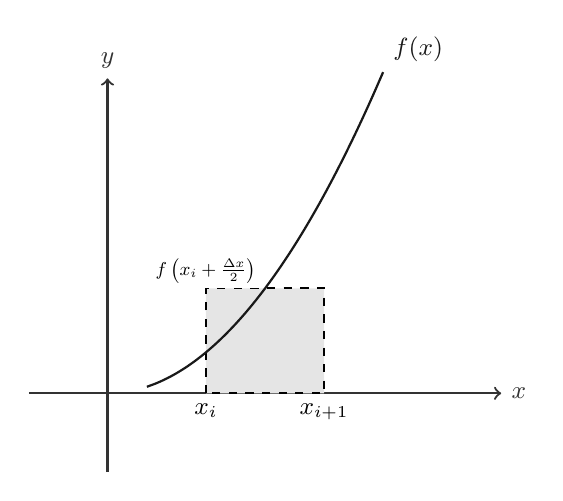
\begin{tikzpicture}[font=\small,thick];

\draw[->, black!80] (-1,0) -- (5,0) node[right] {$x$};
\draw[->, black!80] (0,-1) -- (0,4) node[above] {$y$};
\draw[dashed, fill=gray!20] 
(1.25,0) node[below] {$x_i$} -- 
(1.25,1.3333) node[above, scale=0.75, fill=white, inner sep = 2pt] {$f\left(x_i + \frac{\Delta x}{2}\right)$} -- 
(2.75, 1.3333) -- 
(2.75, 0) node[below] {$x_{i+1}$} -- (1.25,0);
\draw[domain=0.5:3.5, smooth, variable = \x, black!90] plot ({\x}, {0.333*\x*\x}) node[above right]{$f(x)$};
\end{tikzpicture}

\end{document}